\section{Analysis and Motivations}
\label{sec:analysis}
In this section, we analyze the attention map behaviors during the generation time and illustrate how the observations motivate the adaptive attention sparse updates.

\subsection{Cross-step attention similarity}
Existing sparsity methods in DLM, such as SparseD \cite{wang2025sparsed}, are built on the observation that attention patterns exhibit noticeable temporal consistency across inference steps. Based on this observation, they estimate the sparse attention pattern once and reuse it in subsequent denoising steps, thereby avoiding repeated pattern construction overhead. While this assumption is partially valid, we find that it is insufficient to fully characterize attention dynamics in DLLMs. For a query position $i$ at denoising step $s$, we define its attention pattern as $\mathbf{a}_i^{(s)}=\mathrm{Softmax}\left(\frac{\mathbf{q}_i^{(s)}\mathbf{K}^{(s)\top}}{\sqrt{d}}\right)$, which represents the attention distribution of the query token over all key positions at step $s$.

Unlike autoregressive decoding, DLLM inference proceeds through an iterative denoising process, in which the visible context and token certainty evolve continuously across steps. As more tokens become unmasked, the dependency structure of the sequence is gradually refined, and the attention pattern may be reorganized accordingly. In particular, some key positions that are not salient at early steps can become pivotal at later steps.  As illustrated in Figure~\ref{fig:attention_pattern_across_steps}, which compares two groups of nearby denoising steps, the attention patterns are highly consistent within Steps 29--31 and within Steps 39--41, suggesting local reusability across nearby steps. However, comparing these two groups reveals a clear pattern shift: a new pivotal token at key position 95 emerges in Steps 39--41 but is not prominent in Steps 29--31. This indicates that, although the sparse attention pattern can be reused locally, it is not fully stationary throughout denoising.

As further shown in Figure~\ref{fig:cross_step_curve}, the change between two consecutive attention patterns is measured by the KL divergence $D_{\mathrm{KL}}\!\left(\mathbf{a}_i^{(s)} \,\|\, \mathbf{a}_i^{(s-1)}\right)=\sum_{j=1}^{L}\mathbf{a}_{i,j}^{(s)}\log\frac{\mathbf{a}_{i,j}^{(s)}}{\mathbf{a}_{i,j}^{(s-1)}}$. Although many neighboring steps remain relatively similar, there exist several transition steps where the divergence increases sharply, suggesting abrupt changes in the underlying attention structure. This implies that directly reusing a sparse pattern estimated at early steps may lead to stale sparsity decisions: newly important attention links can be missed, while computation is still spent on entries that are no longer critical. These observations motivate us to refresh the sparse attention matrix at some selected anchor steps.





% In DLLMs, the attention computation is formulated as$\mathrm{Out}=\mathrm{Softmax}\left(\frac{QK^\top}{\sqrt{d}}\right)V $, where the corresponding attention scores are defined as $\mathrm{AttnScore}=\mathrm{Softmax}\left(\frac{QK^\top}{\sqrt{d}}\right)$. Here, \(Q,K \in \mathbb{R}^{\mathrm{seq}\times d}\), and \(\mathrm{seq}\) denotes the total sequence length consisting of both the prompt and the generated context. Across all denoising steps, attention is computed over this full sequence. \zz{need polishing}

% for different position tokens, since DLLMs will update the token by unmasking step by step, some position will generate a token and we call this step i as the "tuning point" for the position x\_i. Before this step, this position behaves as decoding, trying to denoising and find the maximal logits and after this step, this position changes to prefilling, which can provide the information for the next steps of token generation.

% For example, referring to Figure 2, during the first two steps, the word tokens are denoised, and then performanced as the prefilling tokens in following steps.
% \xz{1. figure: cross-step similarity and non-similarity case - two figures? one figure?}


% To understand the attention behaviors cross steps, we first measure the attention score cosine similarity across steps. The measurement on the cosine similarity is presented in Figure xxx. Notably, the similarity between steps is \zz{}
% \red{here we need to have some data to present the across-step similarity regular pattern}

% \red{need to update the figure? heatmap}

\begin{figure}[h]
    \centering
    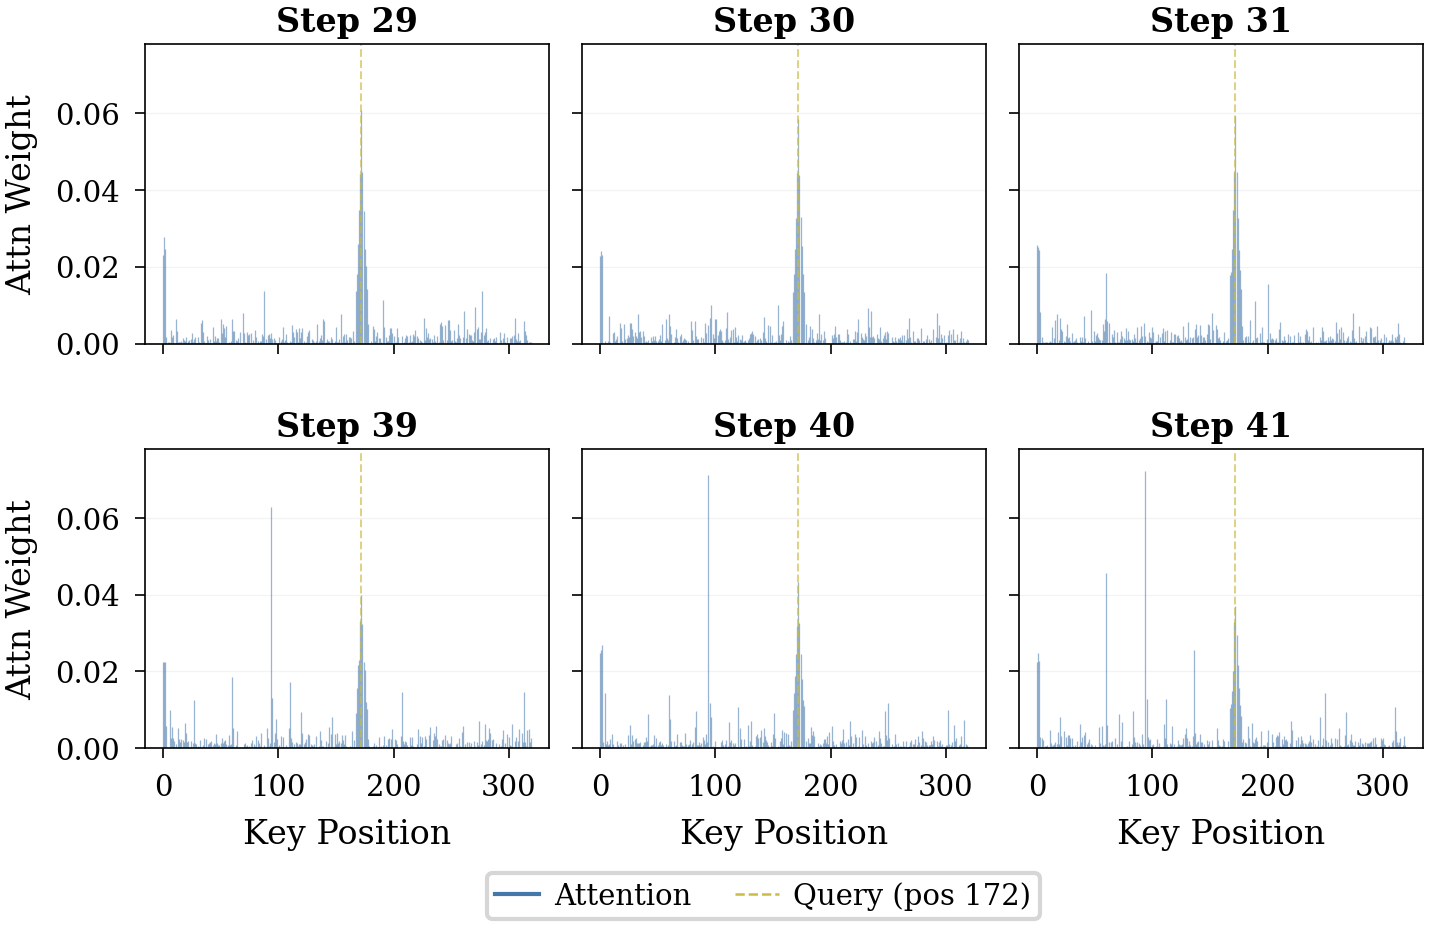
\includegraphics[width=1.0\linewidth]{figures/panels_6step_2x3.png}
    \caption{Attention patterns across different denoising steps.}
    \label{fig:attention_pattern_across_steps}
\end{figure}


\subsection{Head-wise Heterogeneity in Sparse Attention}

Recent sparse DLM methods reduce inference cost by exploiting sparsity during the denoising process. In particular, SparseD\cite{wang2025sparsed} performs sparse attention computation by selecting important token interactions according to token-level attention saliency, while Sparse-dLLM \cite{} improves efficiency through token-level cache eviction. These designs have shown promising efficiency gains in DLM inference. However, they also implicitly treat the token as the primary unit of sparsification, assuming that the importance of a token is largely consistent across attention heads.  We find that this assumption is overly coarse for DLMs.

As shown in Figure~\ref{fig: attention_heterogeneity}(a), even for the same query token, different attention heads can exhibit substantially different attention patterns. 
Some heads focus sharply on a small set of key positions, while others attend more broadly or emphasize entirely different regions. 
This indicates that head-specific behaviors are not merely a secondary effect, but a fundamental property of sparse attention in DLMs. 
Consequently, a unified token-level sparsity decision may be suboptimal: a token that is highly important for one head can be much less informative for another. 
Applying the same sparse mask or compression rule across all heads therefore risks preserving unnecessary computations in some heads while discarding critical attention scores in others.

Moreover, the heterogeneity across heads is reflected not only in attended positions, but also in the concentration of attention mass. 
Figure~\ref{fig: attention_heterogeneity}(b) visualizes the cumulative density of attention scores for different heads. 
We observe that the concentration behaviors vary markedly across heads: some heads are highly concentrated, where preserving only a small fraction of top-scoring entries already retains most of the attention mass, whereas other heads are much more dispersed and require a substantially larger fraction to achieve the same coverage. 
For example, certain heads can preserve around $90\%$ of the attention mass with only about $10\%$ of the entries, while others may require close to $50\%$. 
This suggests that different heads have different compression sensitivities and thus should not be assigned the same sparsity budget.

This observation is qualitatively different from prior token-level acceleration strategies in DLMs. 
SparseD emphasizes that sparse patterns are highly reusable across denoising steps and therefore pre-computes sparse patterns once and reuses them later, while Sparse-dLLM leverages the temporal stability of token saliency to evict low-importance cache entries. 
In contrast, our analysis highlights that, even when sparsity is exploited, the effective compression granularity should be head-aware rather than purely token-level. 
In other words, the key challenge is not only which tokens to preserve, but also how much computation budget each head should receive.

Motivated by this head-wise heterogeneity, we allocate the sparse attention budget globally across heads instead of enforcing a uniform token-level or per-head compression ratio. 
This design allows highly concentrated heads to be compressed more aggressively, while reserving more computation for heads with more dispersed yet important attention patterns. 
As a result, the sparse budget can be utilized more effectively, leading to a better trade-off between efficiency and model quality.


\begin{figure}[t]
    \centering
    \begin{subfigure}[b]{0.49\columnwidth}
        \centering
        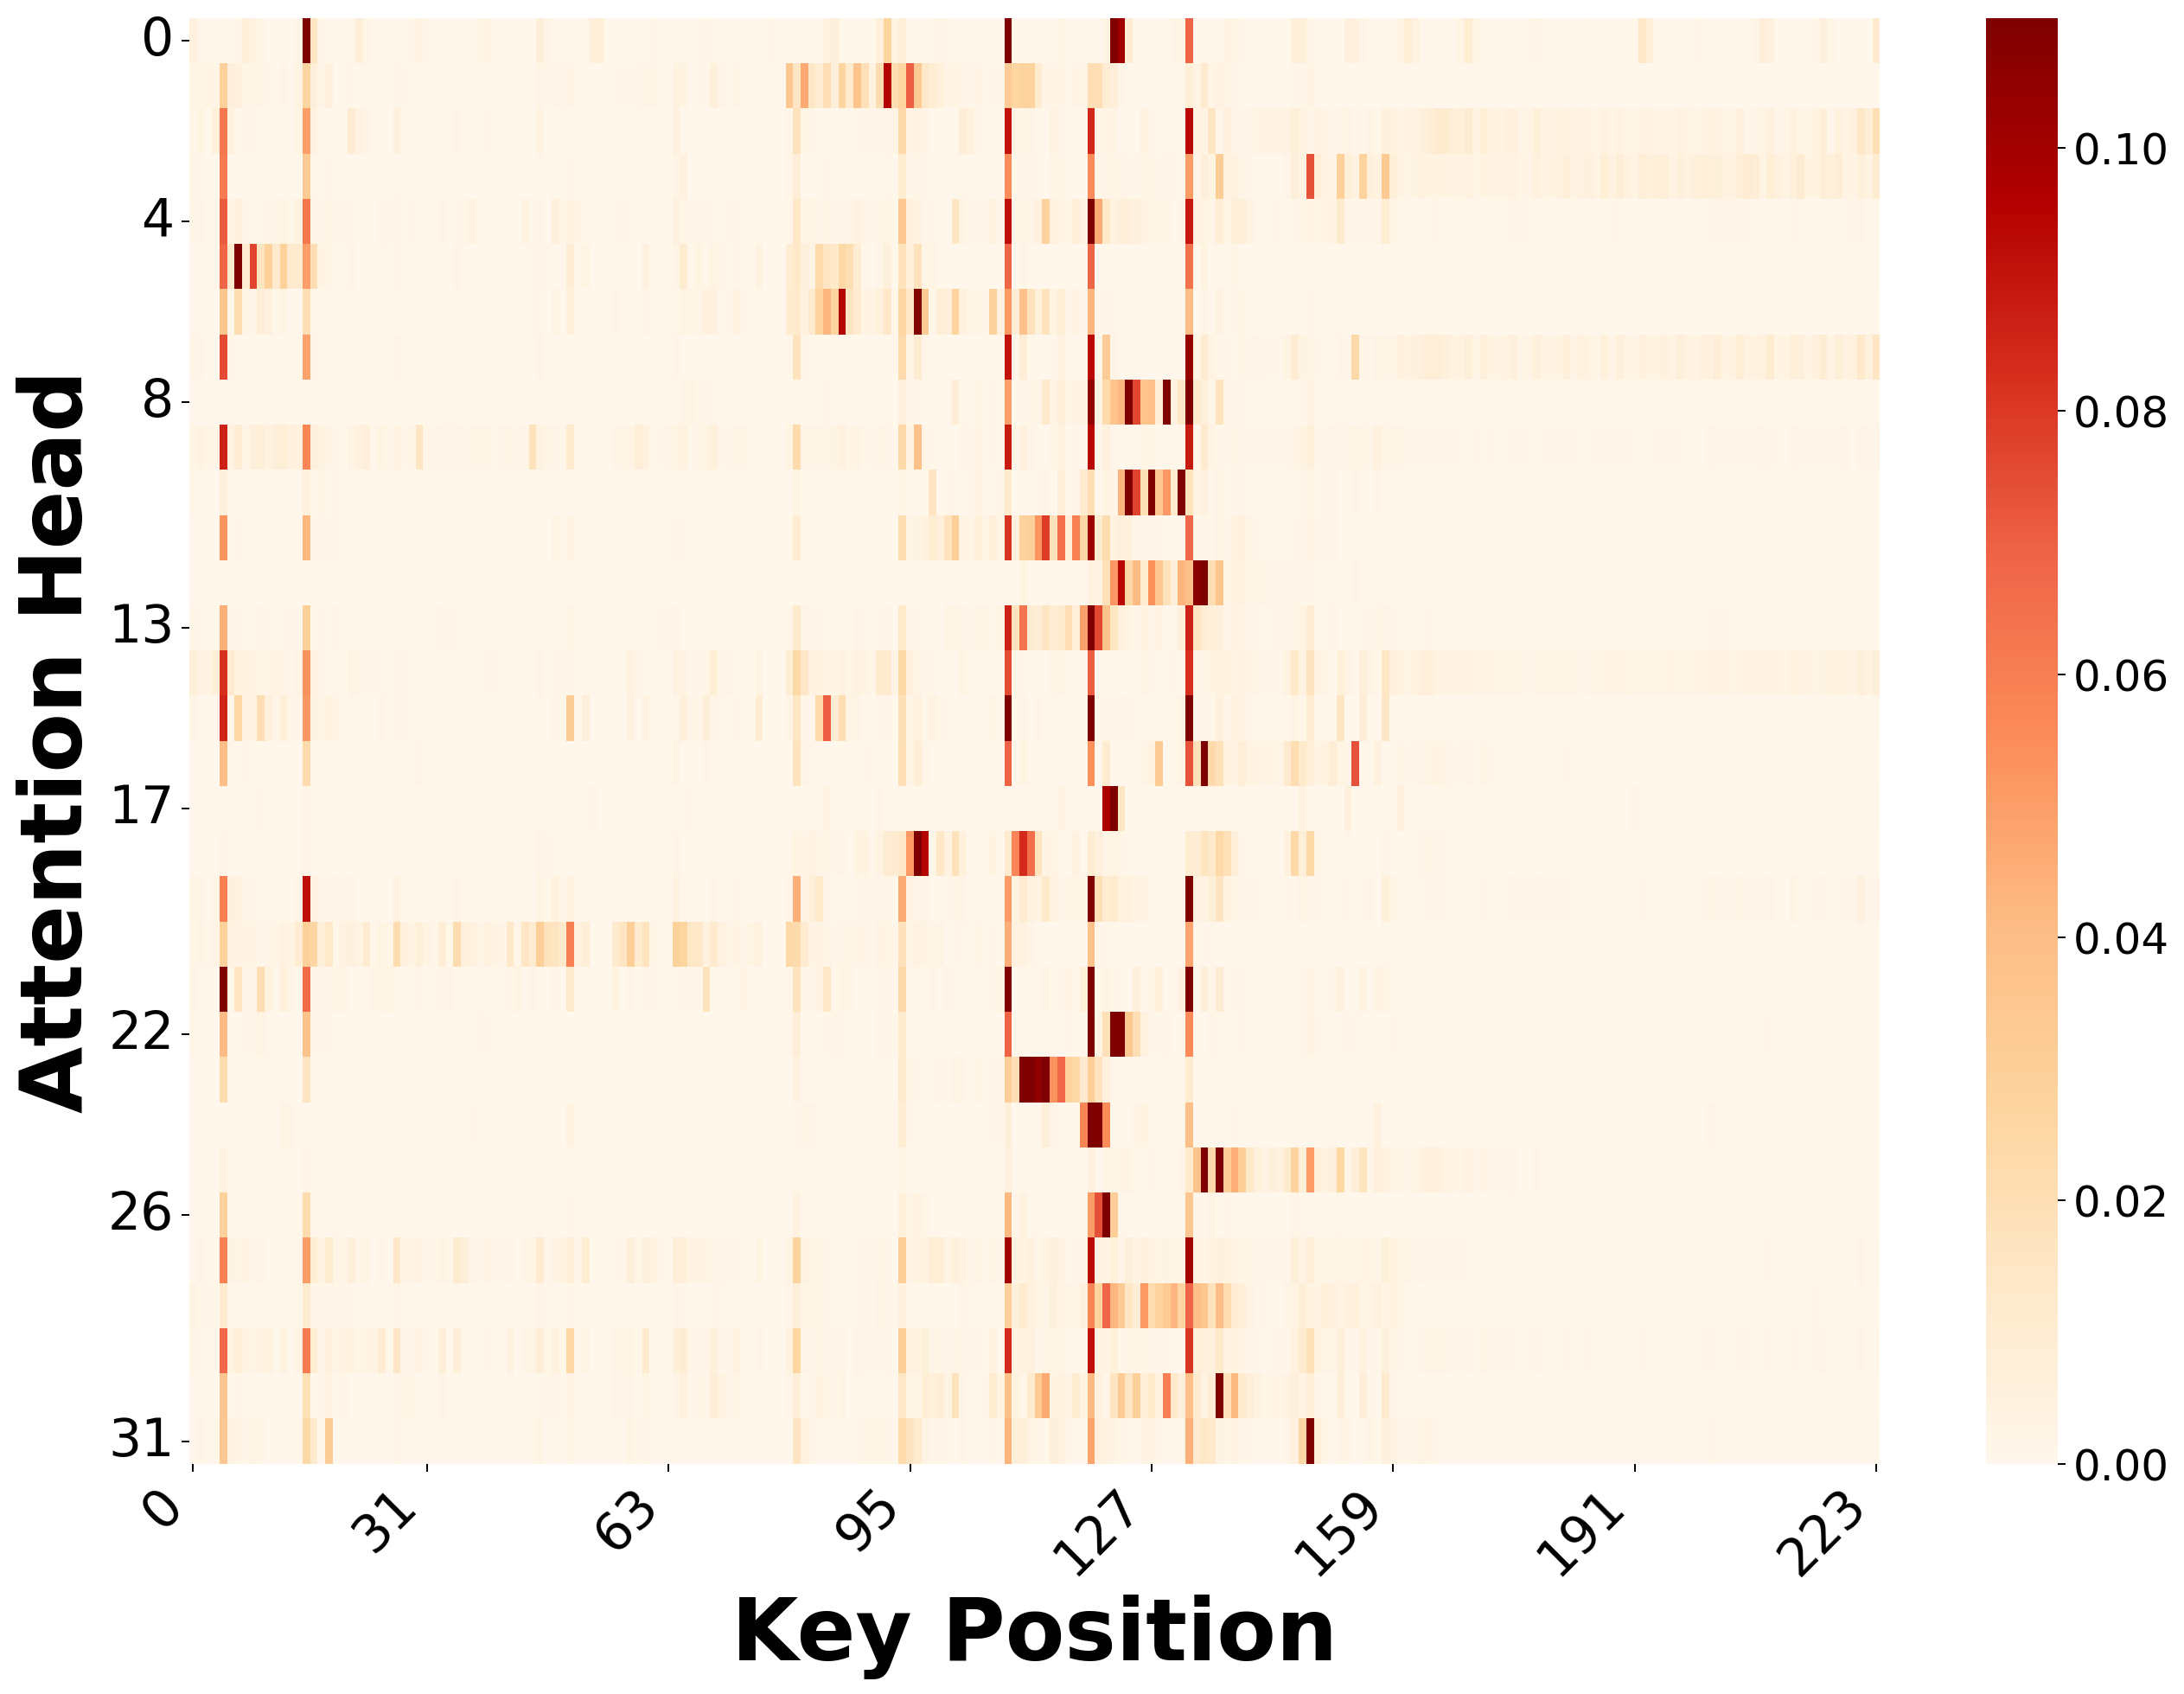
\includegraphics[width=\linewidth]{figures/difference_between_attention_heads.png}
        \caption{Attention patterns of different heads for the same query position, showing head-wise heterogeneity.}
    \end{subfigure}
    \hfill
    \begin{subfigure}[b]{0.49\columnwidth}
        \centering
        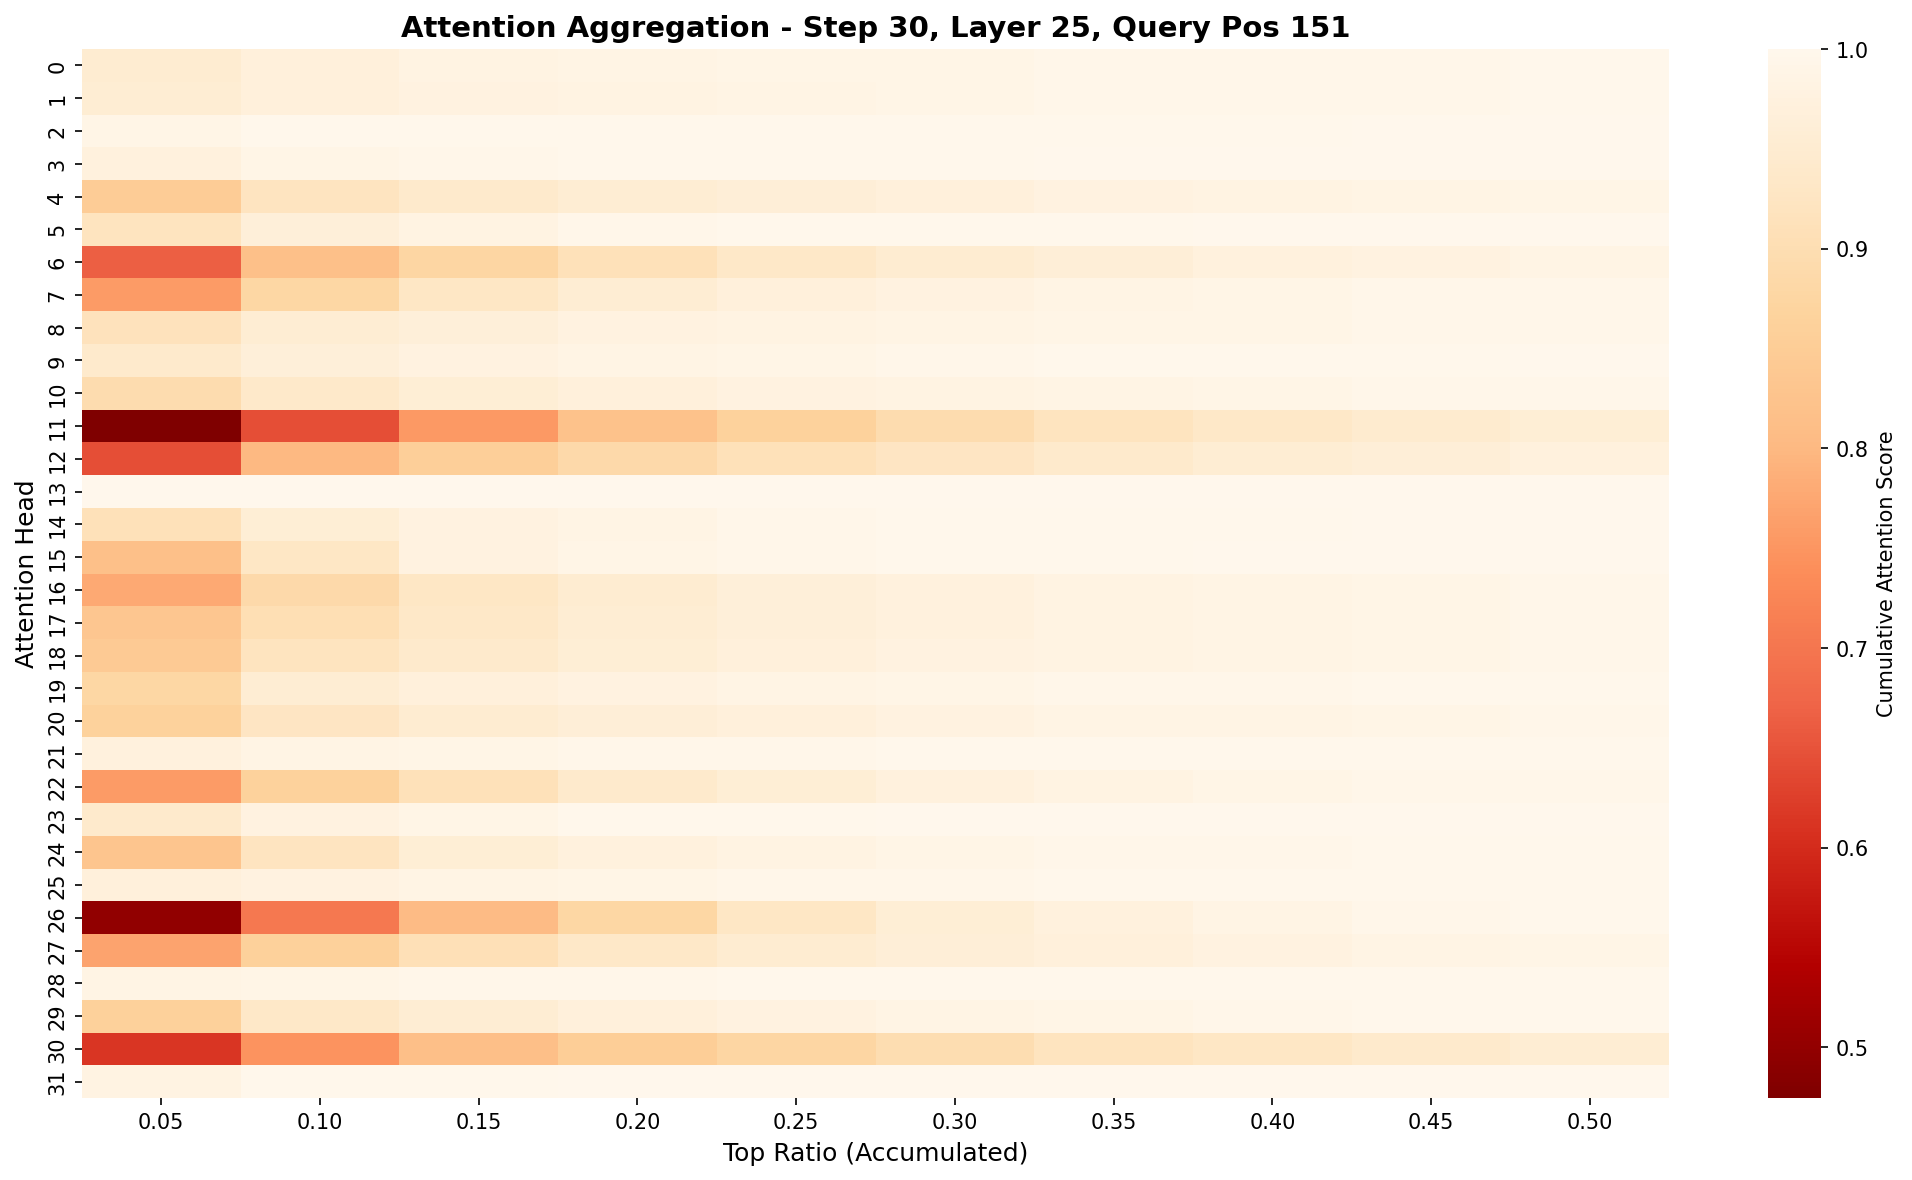
\includegraphics[width=\linewidth]{figures/attention_aggregation_step30_layer25_pos151.png}
        \caption{Cumulative attention mass across heads, illustrating varying concentration levels.}
        \label{fig:budget_cross_head}
    \end{subfigure}

    \caption{Head-wise heterogeneity in attention patterns. (a) Different heads attend to substantially different key positions for the same query. (b) Cumulative attention density varies markedly across heads, indicating different compression sensitivities.}
    \label{fig: attention_heterogeneity}
\end{figure}



% % Motivated by Section 3.2, we proposes a step-aware sparse mask update to reuse the similarity of sparse patterns.

% % Let s be the current diffusion step and L=l+c be the total sequence length. First, we do the attention in the 
% As demonstrated in Section~3.2, attention maps exhibit substantial similarity across consecutive diffusion steps. To exploit this temporal redundancy, we propose a cross-step attention reuse mechanism. Let $s$ denote the current diffusion step, $L$ the total sequence length, $b$ the block size, and $k$ the number of retained blocks per query block. We partition the $\mathbf{Q}, \mathbf{K}, \mathbf{V}$ matrices into blocks of size $b$, yielding $N_b = \lceil L/b \rceil$ blocks along the sequence dimension.

% \textbf{Anchor step computation.} At designated anchor step $i$, we compute full attention using a modified flash attention kernel that simultaneously produces both the attention output and a block-level sparsity mask. For each query block $p$ and key block $q$, we derive a coarse-grained saliency score via block-wise max-pooling over the attention logits:
% \begin{equation}
% \mathbf{M}_{pq} = \max_{(m,n) \in [b] \times [b]} \frac{(\mathbf{Q}_p)_m (\mathbf{K}_q)_n^\top}{\sqrt{d}}
% \end{equation}
% where $\mathbf{M} \in \mathbb{R}^{N_b \times N_b}$ captures the maximum attention affinity within each block pair. For each query block $p$, we retain only the top-$k$ most salient key blocks $\mathcal{I}_p = \mathrm{Top\text{-}k}\!\left(\{\mathbf{M}_{pq}\}_{q=1}^{N_b}\right)$, forming the sparse mask $\mathcal{I} = \{\mathcal{I}_p\}_{p=1}^{N_b}$. The full attention output is computed simultaneously within the fused kernel, so the anchor step jointly returns:
% \begin{equation}
% \mathcal{I},\ \mathbf{O}^{(i)} = \texttt{Modified-Flash-Attn}(\mathbf{Q}, \mathbf{K}, \mathbf{V},\ b,\ k)
% \end{equation}

% \textbf{Non-anchor step computation.} At subsequent steps $i{+}1, i{+}2, \ldots$, we reuse the cached mask indices $\mathcal{I}$ and perform block-sparse attention. For each query block $p$, attention is restricted to the selected key blocks:
% \begin{equation}
% \mathbf{O}^{(i+t)}_p = \mathrm{softmax}\!\left(\frac{\mathbf{Q}_p^{(i+t)} \left[\mathbf{K}_{q}^{(i+t)}\right]_{q \in \mathcal{I}_p}^\top}{\sqrt{d}}\right) \left[\mathbf{V}_{q}^{(i+t)}\right]_{q \in \mathcal{I}_p}
% \end{equation}
% where the superscript $(i{+}t)$ indicates that $\mathbf{Q}, \mathbf{K}, \mathbf{V}$ are freshly computed at step $i{+}t$, while only the sparsity pattern $\mathcal{I}$ is inherited from the anchor step. This reduces the per-step complexity from $\mathcal{O}(L^2)$ to $\mathcal{O}(L \cdot k \cdot b)$, amortizing the cost of full attention over multiple diffusion steps:
% \begin{equation}
% \mathbf{O}^{(i+t)} = \texttt{Block-Sparse-Attn}(\mathbf{Q}^{(i+t)}, \mathbf{K}^{(i+t)}, \mathbf{V}^{(i+t)},\ \mathcal{I})
% \end{equation}

% \textbf{Adaptive re-anchoring.} The sparsity pattern $\mathcal{I}$ derived at an anchor step is not perpetually valid: as illustrated in Figure~\ref{fig:cross_step}, the attention score distribution evolves non-monotonically across diffusion steps, exhibiting pronounced transition points as generation progresses from early denoising to final convergence. Reusing a stale mask beyond these transitions degrades output quality. To balance computational savings against mask fidelity, we introduce a periodic re-anchoring schedule governed by a refresh interval $\Delta$. Every $\Delta$ steps, we designate the current step as a new anchor, recompute full attention via the modified Flash Attention kernel, and refresh the cached mask $\mathcal{I}$. Between consecutive anchors, the mask is frozen and block-sparse attention is applied. The overall procedure, summarized in Algorithm~\ref{alg:step_aware_sparse}, thus amortizes the $\mathcal{O}(L^2)$ cost of full attention over $\Delta$ steps, yielding an average per-step complexity of $\mathcal{O}\!\left(\frac{L^2}{\Delta} + L \cdot k \cdot b\right)$, which approaches $\mathcal{O}(L \cdot k \cdot b)$ for moderate $\Delta$.

% \begin{algorithm}[t]
% \caption{Step-Aware Sparse Attention with Periodic Re-Anchoring}
% \label{alg:step_aware_sparse}
% \begin{algorithmic}[1]
% \Require Diffusion steps $S$, block size $b$, top-$k$ budget, re-anchor interval $\Delta$
% \Ensure Output sequence $\mathbf{O}^{(s)}$ for each step $s = 1, \ldots, S$
% \State $\mathcal{I} \gets \varnothing$ \Comment{Initialize cached sparse mask}
% \For{$s = 1$ \textbf{to} $S$}
%     \State Compute $\mathbf{Q}^{(s)}, \mathbf{K}^{(s)}, \mathbf{V}^{(s)}$ from the current hidden states
%     \If{$s \equiv 1 \pmod{\Delta}$} \Comment{Anchor step}
%         \State $\mathcal{I},\; \mathbf{O}^{(s)} \gets \texttt{Modified-Flash-Attn}\!\left(\mathbf{Q}^{(s)}, \mathbf{K}^{(s)}, \mathbf{V}^{(s)},\; b,\; k\right)$
%         \State \Comment{Full attention + mask extraction}
%     \Else \Comment{Non-anchor step}
%         \State $\mathbf{O}^{(s)} \gets \texttt{Block-Sparse-Attn}\!\left(\mathbf{Q}^{(s)}, \mathbf{K}^{(s)}, \mathbf{V}^{(s)},\; \mathcal{I}\right)$
%         \State \Comment{Sparse attention with cached mask}
%     \EndIf
% \EndFor
% \end{algorithmic}
% \end{algorithm}


% \paragraph{Head-adaptive sparsity budget.}
% Different attention heads in diffusion language models capture distinct structural patterns---some heads attend broadly across the sequence while others focus locally. Imposing a uniform per-head sparsity budget (e.g., a fixed sliding-window size) fails to accommodate this heterogeneity. Instead, we allocate a global sparsity budget across all heads and let each head claim capacity according to its attention saliency. Concretely, let $H$ denote the number of attention heads and $k_h$ the number of retained blocks for head $h$. We constrain the total budget as:
% \begin{equation}
% \sum_{h=1}^{H} k_h = K_{\text{total}}, \quad k_h \geq k_{\min},
% \label{eq:budget}
% \end{equation}
% where $K_{\text{total}}$ is the aggregate block budget across all heads and $k_{\min}$ is a minimum allocation that guarantees each head retains at least a baseline level of context. At each anchor step, we rank heads by their cumulative block-level saliency scores $\sum_{p,q} \mathbf{M}^{(h)}_{pq}$ and distribute the remaining budget $K_{\text{total}} - H \cdot k_{\min}$ proportionally to heads with higher total saliency, allowing attention-heavy heads to retain more key blocks while pruning redundant ones aggressively.

% \paragraph{Customized Triton kernels.}
% To realize the above scheme efficiently on GPU, we implement two fused Triton kernels. The \texttt{Modified-Flash-Attn} kernel extends standard Flash Attention~\citep{dao2022flashattention} to emit the block-level saliency matrix $\mathbf{M}$ as a byproduct of the forward pass, producing both the full attention output $\mathbf{O}$ and the sparse mask $\mathcal{I}$ in a single kernel launch without redundant recomputation of the attention logits. The \texttt{Block-Sparse-Attn} kernel consumes the cached mask indices $\mathcal{I}$ and performs gather-based block-sparse matrix multiplication, loading only the selected key--value blocks into shared memory. Together, the two kernels eliminate the need for any materialized $L \times L$ attention matrix, keeping peak memory at $\mathcal{O}(L \cdot k \cdot b)$ throughout both anchor and non-anchor steps.

\section{Methodology}
\label{sec:method}

We present \textbf{Step-dLLM}, an efficient inference framework for diffusion language models. The key observation (Section~\ref{sec:analysis}) is that attention maps change slowly across consecutive diffusion steps, yet vary at different rates throughout the generation process. Step-dLLM exploits this structure through three integrated components: (i)~a \emph{cross-step mask reuse} scheme that amortizes the cost of identifying sparse patterns (Section~\ref{sec:mask_reuse}), (ii)~a \emph{head-adaptive budget} that allocates sparsity non-uniformly across attention heads (Section~\ref{sec:mask_construction}), and (iii)~\emph{fused Triton kernels} that make both anchor and non-anchor steps hardware-efficient (Section~\ref{sec:kernels}). Figure~\ref{fig:step_dllm_overview} provides an overview.

\begin{figure}[t]
    \centering
    \includegraphics[width=0.95\linewidth]{figures/StepdLLM.png}
    \caption{Overview of \textbf{Step-dLLM}. Anchor steps compute full attention and extract a block-sparse mask via a fused kernel. Non-anchor steps reuse the cached mask with fresh $\mathbf{Q}, \mathbf{K}, \mathbf{V}$, reducing per-step cost from $\mathcal{O}(L^2)$ to $\mathcal{O}(L \cdot k \cdot b)$. The mask is periodically refreshed every $\Delta$ steps.}
    \label{fig:step_dllm_overview}
\end{figure}

%% ----------------------------------------------------------------
\subsection{Cross-Step Sparse Mask Reuse}
\label{sec:mask_reuse}

The per-step $\mathcal{O}(L^2)$ cost of full bidirectional attention is the dominant bottleneck in dLLM inference. Our key observation (Section~\ref{sec:analysis}) is that, although the attention maps evolve across diffusion steps, adjacent steps share highly similar block-level sparsity structures (Figure~\ref{fig:cross_step}). This motivates a simple strategy: \emph{compute the sparse mask once, then reuse it for several subsequent steps}, amortizing the cost of mask identification over a group of steps.

Formally, let $b$ denote the block size and $N_b = \lceil L/b \rceil$ the number of blocks. We partition the $S$ diffusion steps into consecutive groups of size $\Delta$. Within each group, the first step serves as the \emph{anchor} and the remaining $\Delta{-}1$ steps reuse the anchor's mask.

\paragraph{Anchor steps} compute full attention and simultaneously extract a block-level sparsity mask $\mathcal{I}$ (construction detailed in Section~\ref{sec:mask_construction}), both produced by a single fused kernel launch with no redundant recomputation:
\begin{equation}
    \mathcal{I},\ \mathbf{O}^{(s)} = \texttt{Modified-Flash-Attn}(\mathbf{Q}^{(s)}, \mathbf{K}^{(s)}, \mathbf{V}^{(s)},\ b).
\end{equation}

\paragraph{Non-anchor steps} freeze the cached mask $\mathcal{I}$ and restrict attention to the selected blocks. Note that only the sparsity \emph{pattern} is inherited---the queries, keys, and values are freshly computed from the current step's hidden states, so the attention \emph{weights} remain faithful to the evolving token representations:
\begin{equation}
    \mathbf{O}^{(s)} = \texttt{Block-Sparse-Attn}(\mathbf{Q}^{(s)}, \mathbf{K}^{(s)}, \mathbf{V}^{(s)},\ \mathcal{I}).
\end{equation}

The mask is refreshed every $\Delta$ steps, bounding the staleness of $\mathcal{I}$ and accommodating the non-stationary nature of the attention distribution. This yields an average per-step complexity of $\mathcal{O}\!\bigl(\frac{L^2}{\Delta} + L \cdot k \cdot b\bigr)$, which approaches $\mathcal{O}(L \cdot k \cdot b)$ for moderate $\Delta$. The complete procedure is summarized in Algorithm~\ref{alg:step_aware_sparse}.

\begin{algorithm}[t]
\caption{Step-dLLM Inference}
\label{alg:step_aware_sparse}
\begin{algorithmic}[1]
\Require Diffusion steps $S$, block size $b$, global budget $K_{\text{total}}$, per-head minimum $k_{\min}$, re-anchor interval $\Delta$, number of heads $H$
\Ensure Output $\mathbf{O}^{(s)}$ for each step $s = 1, \ldots, S$
\State $\mathcal{I} \gets \varnothing$ \Comment{Cached block-sparse mask across all heads}
\For{$s = 1$ \textbf{to} $S$}
    \State Compute $\mathbf{Q}^{(s)}, \mathbf{K}^{(s)}, \mathbf{V}^{(s)} \in \mathbb{R}^{H \times L \times d}$ from current hidden states
    \If{$\mathcal{I} = \varnothing$ \textbf{or} $s \equiv 1 \pmod{\Delta}$} \Comment{Anchor step}
        \State $\mathbf{M},\; \mathbf{O}^{(s)} \gets \texttt{Modified-Flash-Attn}\!\left(\mathbf{Q}^{(s)}, \mathbf{K}^{(s)}, \mathbf{V}^{(s)},\; b\right)$
            \Comment{$\mathbf{M} \in \mathbb{R}^{H \times N_b \times N_b}$, all heads in parallel}
        \State $S_h \gets \sum_{p,q} \mathbf{M}^{(h)}_{pq}$ for $h = 1, \ldots, H$
            \Comment{Per-head cumulative saliency}
        \State Allocate $\{k_h\}_{h=1}^{H}$ from $K_{\text{total}}$ proportionally to $\{S_h\}$ subject to $k_h \geq k_{\min}$ \Comment{Eq.~\eqref{eq:budget}}
        \State $\mathcal{I}^{(h)}_p \gets \mathrm{Top\text{-}k_h}\!\left(\{\mathbf{M}^{(h)}_{pq}\}_{q=1}^{N_b}\right)$ for all $h, p$
            \Comment{Extract sparse mask}
    \Else \Comment{Non-anchor step}
        \State $\mathbf{O}^{(s)} \gets \texttt{Block-Sparse-Attn}\!\left(\mathbf{Q}^{(s)}, \mathbf{K}^{(s)}, \mathbf{V}^{(s)},\; \mathcal{I}\right)$
            \Comment{All heads in parallel, mask $\mathcal{I}$ reused}
    \EndIf
\EndFor
\end{algorithmic}
\end{algorithm}

%% ----------------------------------------------------------------
\subsection{Block-Sparse Mask Construction with Head-Adaptive Budget}
\label{sec:mask_construction}
%% ----------------------------------------------------------------

We now describe how the sparsity mask $\mathcal{I}$ is constructed at each anchor step. The procedure involves two stages: computing block-level saliency scores and allocating a non-uniform budget across heads.

\paragraph{Block-level saliency scoring.}
Let $L$ denote the total sequence length and $b$ the block size. We partition $\mathbf{Q}, \mathbf{K}, \mathbf{V}$ into $N_b = \lceil L/b \rceil$ blocks along the sequence dimension. For each attention head $h$, query block $p$, and key block $q$, we compute a coarse saliency score via block-wise max-pooling over the attention logits:
\begin{equation}
    \mathbf{M}^{(h)}_{pq} = \max_{(m,n) \in [b] \times [b]} \frac{(\mathbf{Q}^{(h)}_p)_m (\mathbf{K}^{(h)}_q)_n^\top}{\sqrt{d}},
\end{equation}
where $\mathbf{M}^{(h)} \in \mathbb{R}^{N_b \times N_b}$ captures the maximum attention affinity within each block pair for head $h$. This scoring is performed as a byproduct of the full attention computation inside the fused \texttt{Modified-Flash-Attn} kernel (Section~\ref{sec:kernels}), incurring no additional pass over the data.

\paragraph{Head-adaptive budget allocation.}
Different heads serve distinct structural roles: some attend globally across the full sequence while others focus on narrow local windows. Assigning a uniform block budget $k$ to every head either wastes capacity on locally-focused heads or starves globally-attending ones. We therefore impose a global budget shared across all $H$ heads:
\begin{equation}
    \sum_{h=1}^{H} k_h = K_{\text{total}}, \quad k_h \geq k_{\min},
    \label{eq:budget}
\end{equation}
where $K_{\text{total}}$ controls the overall computation--quality trade-off and $k_{\min}$ ensures every head retains a minimum context window. The surplus budget $K_{\text{total}} - H \cdot k_{\min}$ is distributed proportionally to each head's cumulative saliency $S_h = \sum_{p,q} \mathbf{M}^{(h)}_{pq}$, allowing attention-heavy heads to retain more key blocks while aggressively pruning redundant ones. Given the per-head budget $k_h$, the mask for head $h$ is:
\begin{equation}
    \mathcal{I}^{(h)}_p = \mathrm{Top\text{-}k_h}\!\left(\{\mathbf{M}^{(h)}_{pq}\}_{q=1}^{N_b}\right), \quad \mathcal{I}^{(h)} = \{\mathcal{I}^{(h)}_p\}_{p=1}^{N_b}.
\end{equation}
This formulation keeps the total computational envelope fixed at $K_{\text{total}}$ blocks while letting the distribution adapt to each head's functional demands.

\subsection{Fused Triton Kernel Implementation}
\label{sec:kernels}

The algorithmic gains described above are only realized if the underlying kernels can efficiently execute both full and sparse attention without materializing the $L \times L$ attention matrix. We implement two complementary fused kernels in Triton~\citep{tillet2019triton}. The first, \texttt{Modified-Flash-Attn}, extends Flash Attention~\citep{dao2022flashattention} to emit the block-level saliency matrix $\mathbf{M}^{(h)}$ as a byproduct of the forward pass: as the kernel tiles over key blocks in its inner loop, it maintains a running per-block maximum of the attention logits at negligible additional cost, so that a single kernel launch produces both the full attention output $\mathbf{O}$ and all saliency scores needed for mask construction without any redundant recomputation. The second, \texttt{Block-Sparse-Attn}, consumes the cached mask indices $\mathcal{I}^{(h)}$ and performs gather-based block-sparse attention---for each query block $p$, only the $k_h$ key--value blocks indicated by $\mathcal{I}^{(h)}_p$ are loaded into shared memory while all unselected blocks are skipped entirely, yielding wall-clock speedups proportional to the sparsity ratio $k_h / N_b$. Together, the two kernels keep peak memory at $\mathcal{O}(L \cdot k \cdot b)$ throughout both anchor and non-anchor steps.